\section{Span}
% 1.6
\textbf{Spannet} er den del af vektorrummet, som linearkombinationen af en given mængde vektorer dækker over. 
%
\begin{defn}{}{}
%
For en ikke-tom mængde vektorer $\S = {\mathbf{u}_1, \mathbf{u}_2 , \ldots , \mathbf{u}_k }$ i $\R^n$ er spannet af $\S$ mængden af alle linearkombinationer af $\mathbf{u}_1, \mathbf{u}_2 , \ldots , \mathbf{u}_k$ i $\R^n$. 
Denne mængde noteres $\text{span} \{ \S \}$ eller $\text{span}\{ \mathbf{u}_1, \mathbf{u}_2 , \ldots , \mathbf{u}_k \}$.
%
\end{defn}
%
\noindent
Mængden som indeholder vektorerne som udgør spannet kaldes for en \textbf{mængde af generatorer}.
\\
%
%%%%%%%%%%%%%%%%%%%%%%%%%%%%%%%%%%%%%%%%%%%%%%%%%%%%%%%%%%%%%%%%%%%%%%%%
%
\begin{eks}
%
Givet mængderne af vektorer $\S_1$ og $\S_2$, kan $\text{span}\{\S_1 \}$ og $\text{span}\{\S_2 \}$ findes.
%
\begin{align*}
\S_1 &= \left\{
\begin{bmatrix}
           -1 \\
           1 \\
\end{bmatrix}
,
\begin{bmatrix}
           2 \\
           -2 \\
\end{bmatrix}
\right\}
= \left\{ \mathbf{u}_1, \mathbf{u}_2 \right\}
\\
\S_2 &= \left\{
\begin{bmatrix}
           -1 \\
           1 \\
\end{bmatrix}
,
\begin{bmatrix}
           2 \\
           -2 \\
\end{bmatrix}
,
\begin{bmatrix}
           1 \\
           2 \\
\end{bmatrix}
\right\}
= \left\{ \mathbf{u}_1, \mathbf{u}_2,  \mathbf{u}_3 \right\}
\end{align*}
%
Spannet for $\S_1$ bliver derfor:
%
\begin{align*}
\text{span}\{\S_1 \} =
\left\{ x_1 
\begin{bmatrix}
           -1 \\
           1 \\
\end{bmatrix} 
+ x_2
\begin{bmatrix}
           2 \\
           -2 \\
\end{bmatrix}
\right\}.
\end{align*}
%
Som det fremgår geometrisk på figur \ref{span_eks}, er $\text{span}\{\S_1 \}$ en ret linje. 
Eftersom $\mathbf{u}_2$ er en mulig linearkombination af $\mathbf{u}_1$, kan dette reduceres til  
%
\begin{align*}
\text{span}\{\S_1 \} =
\left\{ x_1 
\begin{bmatrix}
           -1 \\
           1 \\
\end{bmatrix} 
\right\}.
\end{align*}
%
Mængden $\S_2$ kan derfor reduceres til $\S_2=\{ \mathbf{u}_1, \mathbf{u}_3 \}$. 
Spannet for $\S_2$ er derfor
%
\begin{align*}
\text{span}\{\S_2 \} = 
\left\{ x_1 
\begin{bmatrix}
           -1 \\
           1 \\
\end{bmatrix} 
+ x_2
\begin{bmatrix}
           1 \\
           2 \\
\end{bmatrix}
\right\}
= \R^2,
\end{align*}
%
da den dækker alle punkter i planen. 
% Eventuelt planet xD
Dette gør den, da det er muligt at besøge alle punkter ved at indføre passende værdier for $x_1$ og $x_2$.
%
% Skal sættes rigtigt inden aflevering!
\begin{figure}[h!]
%
\centering
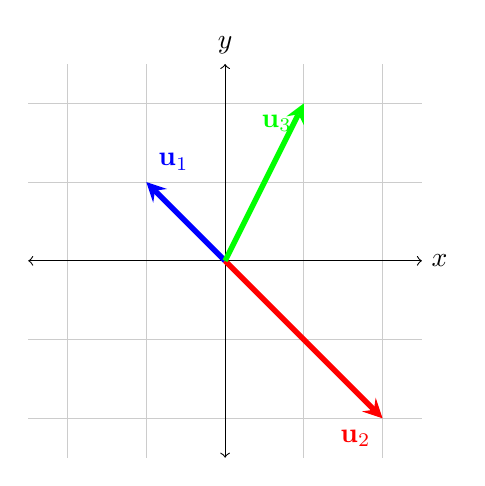
\begin{tikzpicture}
  \draw[thin,gray!40] (-2.5,-2.5) grid (2.5,2.5);
  \draw[<->] (-2.5,0)--(2.5,0) node[right]{$x$};
  \draw[<->] (0,-2.5)--(0,2.5) node[above]{$y$};
  \draw[line width=2pt,blue,-stealth](0,0)--(-1,1) node[anchor=south west]{$\boldsymbol{\mathbf{u}_1}$};
  \draw[line width=2pt,red,-stealth](0,0)--(2,-2) node[anchor=north east]{$\boldsymbol{\mathbf{u}_2}$};
  \draw[line width=2pt,green,-stealth](0,0)--(1,2) node[anchor=north east]{$\boldsymbol{\mathbf{u}_3}$};
\end{tikzpicture}
%
\caption{Grafisk illustration af mængderne $\S_1 \subset \S_2$.}
\label{span_eks}
\end{figure}
%
\end{eks}
%
%%%%%%%%%%%%%%%%%%%%%%%%%%%%%%%%%%%%%%%%%%%%%%%%%%%%%%%%%%%%%%%%%%%%%%%%
%
Typisk bruges span til at undersøge, hvorvidt en given vektor er i spannet for en vektormængde. 
Dette gøres ved at undersøge om en vektor kan konstrueres som linearkombination af vektorerne i mængden, hvilket undersøges ved hjælp af rækkereduktionsalgoritmen. 
\\
%
%%%%%%%%%%%%%%%%%%%%%%%%%%%%%%%%%%%%%%%%%%%%%%%%%%%%%%%%%%%%%%%%%%%%%%%%
%
\begin{eks}
%
Det skal undersøges, hvorvidt vektor $\mathbf{u}$ er i spannet for $\S_1$. 
Givet
\begin{align*}
\mathbf{v}= \begin{bmatrix}
           -1 \\
           2 \\
           3 \\
\end{bmatrix} 
\text{      }
\text{span}\{\S \} =
\left\{ 
\begin{bmatrix}
           1 \\
           2 \\
           1 \\
\end{bmatrix} 
,
\begin{bmatrix}
           1 \\
           1 \\
           0 \\
\end{bmatrix}
,
\begin{bmatrix}
           1 \\
           -1 \\
           -2 \\
\end{bmatrix}
\right\}.
\end{align*}
%
Dette opskrives nu som total-matricen
%
\begin{align*}
A=&
\begin{blockarray}{ccccc}
\mathbf{u}_1 & \mathbf{u}_2 & \mathbf{u}_3 & \mathbf{v} \\
\begin{block}{[ccc|c]c}
  1 & 1 & 1 & -1 \\
  2 & 1 & -1 & 2 \\
  1 & 0 & -2 & 3 \\
\end{block}
\end{blockarray} 
\end{align*}
%
Denne omskrives nu til trappeform
%
\begin{align*}
\xrightarrow[R_3 \rightarrow R_3-R_1]{R_2 \rightarrow R_2-2R_1}&
\begin{blockarray}{ccccc}
\mathbf{u}_1 & \mathbf{u}_2 & \mathbf{u}_3 & \mathbf{v} \\
\begin{block}{[ccc|c]c}
  1 & 1 & 1 & -1 \\
  0 & -1 & -3 & 4 \\
  0 & -1 & -3 & 4 \\
\end{block}
\end{blockarray} \\
%
\xrightarrow{R_3 \rightarrow R_3-R_2}&
\begin{blockarray}{ccccc}
\mathbf{u}_1 & \mathbf{u}_2 & \mathbf{u}_3 & \mathbf{v} \\
\begin{block}{[ccc|c]c}
  \hlight{1} & 1 & 1 & -1 \\
  0 & \hlight{-1} & -3 & 4 \\
  0 & 0 & 0 & 0 \\
\end{block}
\end{blockarray} 
\end{align*}
%
Ud fra dette ses det, at $\mathbf{v}$ er i $\text{span}\{\S \}$.
%
\end{eks}
%
%%%%%%%%%%%%%%%%%%%%%%%%%%%%%%%%%%%%%%%%%%%%%%%%%%%%%%%%%%%%%%%%%%%%%%%%
%
Egenskaberne vedrørende spannet kan udtrykkes på forskellige måder, hvilket leder til følgende sætning:
% 
\begin{thm}{}{spaneqv}
%
De følgende udsagn om en $m \times n$ matrix $A$ er ækvivalente:
%
\begin{enumerate}[label=(\alph*)]
\item Spannet af søjlerne i $A$ er $\R^m$.
\item Matricen $A\mathbf{x}=\mathbf{b}$ har mindst én løsning for alle $b$ i $\R^m$.
\item Rangen af $A$ er antallet af rækker $m$.
\item Den reducerede trappeform har ingen nulrækker.
\item Der er pivot-indgang i hver række i $A$. 
\end{enumerate}
%
\end{thm}
%
%
\begin{proof}
%
Udsagn (a) og (b) er ækvivalente, eftersom det er en forudsætning, at der kan skabes en linear kombination af $A\mathbf{x} =\mathbf{b}$ for ethvert $\mathbf{b}$ i $\R^m$, da det netop er definitionen af spannet, der dækker $\R^m$. 
%
Hvis der ikke er nogle nul-rækker i den reducerede trappeform, følger det, at $\text{rang}\{A\}$ er $m$, hvorfor (c) og (d) er ækvivalente. 
Eftersom matrixen er på reduceret trappeform, er denne derfor ækvivalent med (e).
\\\\
Det skal nu bevises at (b) og (c) er ækvivalente. 
Lad $B$ være den reducerede trappeform af $A$, og $\mathbf{e}_m$ er standard vektoren
%
\begin{align*}
\mathbf{\mathbf{e}_m} = \begin{bmatrix}
		0 \\
        \vdots \\
        0 \\
        1 
\end{bmatrix}
\end{align*}
%
i $\R^m$. 
Gennem rækkereduktionsalgoritmen kan $A$ transformeres til $B$. 
Da disse række er reversible, følger det, at der findes en sekvens af rækkeopperationer, som kan transformere $B$ til $A$.
Hvis disse opperationer udføres på totalmatricen 
$[B \text{    } \mathbf{e}_m]$ 
for at konstruere matricen 
$[A \text{    } \mathbf{d}]$, 
$\mathbf{d} \in \R^n$, 
så følger det, at ligningssystemet $A\mathbf{x}=\mathbf{
d}$ er ækvivalent med $B\mathbf{x}=\mathbf{e}_m$.
\\\\
Hvis (b) er sand, følger det, at de to ligningssystemer er konsistente. 
Det følger derfor af sætning \ref{thm:konsistens}, at den sidste række ikke kan være en nulrække, da standardvektoren $\mathbf{e}_m$ vil have pivotindgang i sidste søjle og derfor vil ligningssystemet være inkonsistent.
Dermed er $rang(A)=m$, hvilket leder til (c).
% Dette kan eventuelt forklares dybere xD
\\\\
Antag, at (c) er sand. 
Lad $[B \text{    }| \mathbf{c}]$ 
være den reducerede trappeform af 
$[A \text{    } | \mathbf{b}]$.
Eftersom $A$ har rangen $m$, følger det, at der ikke findes en nulrække i $B$.
Derfor kan $[B \text{    } \mathbf{c}]$ ikke indeholde en nulrække, hvis eneste nulindgang er i sidste søjle. 
Det følger derfor jævnfør sætning \ref{thm:konsistens}, at $A\mathbf{x}=\mathbf{b}$ er konsistent $\forall \mathbf{b}$, hvilket beviser at (b) og (c) er ækvivalente.
%
\end{proof}
\\
%
%%%%%%%%%%%%%%%%%%%%%%%%%%%%%%%%%%%%%%%%%%%%%%%%%%%%%%%%%%%%%%%%%%%%%%%%
%
Når det skal afgøres, hvorvidt en vektor tilhører et givet span, gælder sætning \ref{thm:span}.
%
\begin{thm}{}{span}
%
Lad $\S =  \{ \mathbf{u}_1, \mathbf{u}_2 , \ldots , \mathbf{u}_k \}$ være en mængde vektorer i $\R^n$, og lad $\mathbf{v}$ være en vektor i $\R^n$.
Så er $\text{span}\{ \mathbf{u}_1, \mathbf{u}_2 , \ldots , \mathbf{u}_k , \mathbf{v}\} =\text{span}\{\S\}$, hvis og kun, hvis $\mathbf{v}$ tilhører $\text{span}\{\S\}$.
%
\end{thm}
%
%
\begin{proof}
%
Antag, at $\mathbf{v}$ er i $\text{span}\{\S\}$. Så er $\mathbf{v}$ en linearkombination af $\S$, hvilket kan opskrives som $\mathbf{v}=a_1\mathbf{u}_1+a_2\mathbf{u}_2+ \ldots + a_k\mathbf{u}_k$, hvor $a_1,a_2,\ldots, a_k$ er skalarer. 
Hvis en vektor $\mathbf{w}$ er i $\text{span}\{ \mathbf{u}_1, \mathbf{u}_2 , \ldots , \mathbf{u}_k , \mathbf{v}\}$, 
kan denne opskrives $\mathbf{w}=c_1\mathbf{u}_1+c_2\mathbf{u}_2+ \ldots + c_k\mathbf{u}_k+b\mathbf{v}$, hvor $c_1,c_2,\ldots, c_k, b$ er skalarer.
Ved substitution af $\mathbf{v}$ med $\{ \mathbf{u}_1, \mathbf{u}_2 , \ldots , \mathbf{u}_k , \mathbf{v}\}$ vides det, at $\mathbf{w}$ kan opskrives som en linearkombination af $\S$. 
Det gælder endvidere, at alle linearkombinationer i $\S$ også kan dannes fra vektorerne $\mathbf{u}_1,\mathbf{u}_1, \mathbf{u}_2 , \ldots , \mathbf{u}_k , \mathbf{v}$, hvis $\mathbf{v}$ multipliceres med skalaren $0$.
Det følger derfor, at de to mængder har samme span. 
Antag nu, at $v$ ikke er i $\text{span}\{\S\}$. 
Det følger herfra, at $\mathbf{v}$ er i spannet af 
$\{ \mathbf{u}_1,\mathbf{u}_1, \mathbf{u}_2 , \ldots , \mathbf{u}_k , \mathbf{v}\}$, da 
$\mathbf{v}=0\mathbf{u}_1+0\mathbf{u}_2+ \ldots + 0\mathbf{u}_k+1\mathbf{v}$.
Derfor er
$\text{span}\{ \mathbf{u}_1,, \mathbf{u}_2 , \ldots , \mathbf{u}_k \}
\neq
\text{span}\{ \mathbf{u}_1,, \mathbf{u}_2 , \ldots , \mathbf{u}_k , \mathbf{v}\}$, 
da mængderne ikke er ækvivalente, idet kun én af dem indeholder $\mathbf{v}$. 
%
\end{proof}
\\
%
%%%%%%%%%%%%%%%%%%%%%%%%%%%%%%%%%%%%%%%%%%%%%%%%%%%%%%%%%%%%%%%%%%%%%%%%
%
Som det fremgår af overstående gælder det derfor, at enhver løsning i et lineært optimeringsproblem skal findes i spannet for vektorerne i ligningssystemet. 
%